\documentclass[tikz,border=12pt]{standalone}
\usepackage[T1]{fontenc}
\usepackage{mathpazo}
\usepackage{amsmath,amssymb}
\usetikzlibrary{arrows.meta, positioning, calc}

\definecolor{stblue}{HTML}{7B97AD}
\definecolor{rwgold}{HTML}{B8995E}
\definecolor{sage}{HTML}{7A9A7E}
\definecolor{dkbrown}{HTML}{3D3530}
\definecolor{wmgray}{HTML}{7B7067}
\definecolor{cream}{HTML}{F9F6F0}
\definecolor{border}{HTML}{D4C9B8}
\definecolor{terracotta}{HTML}{C47A6A}

\begin{document}
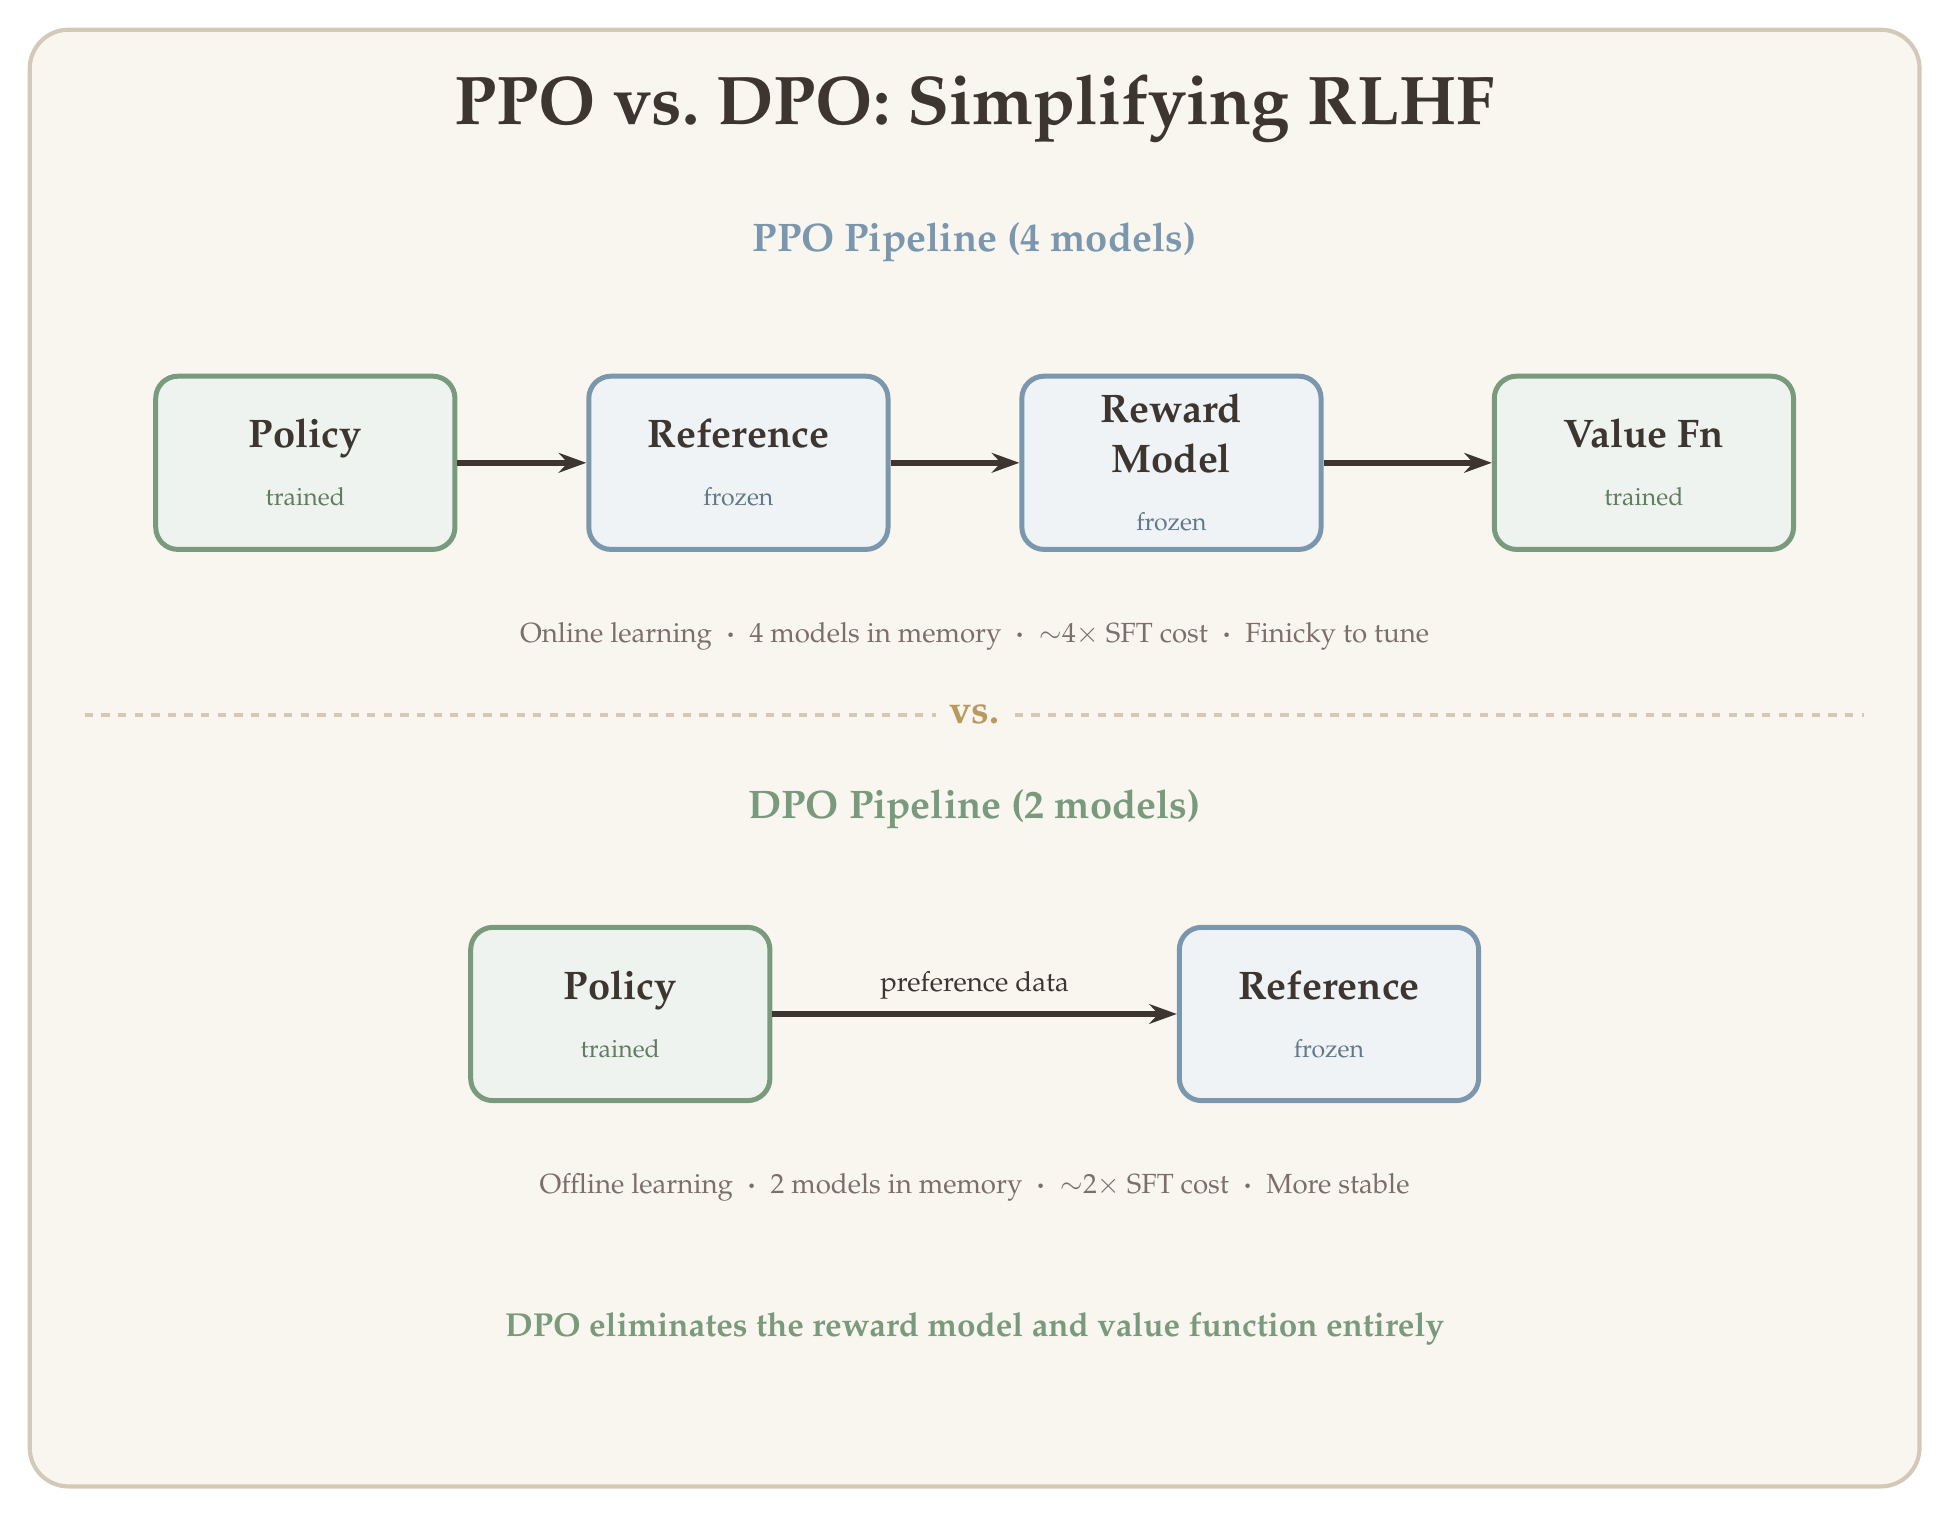
\begin{tikzpicture}[
  >={Stealth[length=3.5mm, width=2.5mm]},
  modelbox/.style 2 args={
    draw=#1, line width=1.8pt, fill=#1!12, rounded corners=8pt,
    minimum width=38mm, minimum height=22mm, font=\Large,
    text=dkbrown, align=center, inner sep=6pt
  },
  arr/.style={->, line width=2pt, dkbrown},
  note/.style={font=\normalsize, text=wmgray, align=center},
]

% Background
\fill[cream, rounded corners=14pt] (-1,-1) rectangle (23,17.5);
\draw[border, rounded corners=14pt, line width=1.5pt] (-1,-1) rectangle (23,17.5);

% Title
\node[font=\Huge\bfseries, text=dkbrown] at (11,16.5)
  {PPO vs.\ DPO: Simplifying RLHF};

% =============================================
% PPO Pipeline
% =============================================
\node[font=\Large\bfseries, text=stblue] at (11,14.8)
  {PPO Pipeline (4 models)};

% Four boxes
\node[modelbox={sage}{}] (pol1) at (2.5,12)
  {\textbf{Policy}\\[3pt]
   \small\color{sage!80!black} trained};

\node[modelbox={stblue}{}] (ref1) at (8,12)
  {\textbf{Reference}\\[3pt]
   \small\color{stblue!80!black} frozen};

\node[modelbox={stblue}{}] (rew) at (13.5,12)
  {\textbf{Reward}\\
   \textbf{Model}\\[3pt]
   \small\color{stblue!80!black} frozen};

\node[modelbox={sage}{}] (val) at (19.5,12)
  {\textbf{Value Fn}\\[3pt]
   \small\color{sage!80!black} trained};

% Arrows between PPO boxes
\draw[arr] (pol1.east) -- (ref1.west);
\draw[arr] (ref1.east) -- (rew.west);
\draw[arr] (rew.east) -- (val.west);

% PPO description
\node[note] at (11,9.8)
  {Online learning\enspace$\boldsymbol{\cdot}$\enspace
   4 models in memory\enspace$\boldsymbol{\cdot}$\enspace
   ${\sim}4{\times}$ SFT cost\enspace$\boldsymbol{\cdot}$\enspace
   Finicky to tune};

% =============================================
% Divider
% =============================================
\draw[dashed, line width=1.5pt, border] (-0.3,8.8) -- (22.3,8.8);
\node[fill=cream, inner sep=5pt, font=\Large\bfseries, text=rwgold] at (11,8.8) {vs.};

% =============================================
% DPO Pipeline
% =============================================
\node[font=\Large\bfseries, text=sage] at (11,7.6)
  {DPO Pipeline (2 models)};

% Two boxes, centered
\node[modelbox={sage}{}] (pol2) at (6.5,5)
  {\textbf{Policy}\\[3pt]
   \small\color{sage!80!black} trained};

\node[modelbox={stblue}{}] (ref2) at (15.5,5)
  {\textbf{Reference}\\[3pt]
   \small\color{stblue!80!black} frozen};

% Arrow with label
\draw[arr] (pol2.east) -- node[above, font=\normalsize, text=dkbrown, yshift=1pt]
  {preference data} (ref2.west);

% DPO description
\node[note] at (11,2.8)
  {Offline learning\enspace$\boldsymbol{\cdot}$\enspace
   2 models in memory\enspace$\boldsymbol{\cdot}$\enspace
   ${\sim}2{\times}$ SFT cost\enspace$\boldsymbol{\cdot}$\enspace
   More stable};

% Bottom annotation
\node[font=\large\bfseries, text=sage] at (11,1)
  {DPO eliminates the reward model and value function entirely};

\end{tikzpicture}
\end{document}
